\chapter{Positive Kaon Cross Section Measurement}\label{ch:KaonXS}

In this chapter, we show the result of the thin slice method to measure  the ($K^+$-Ar) total hadronic cross section. In Section \ref{ch:KaonXSRaw}, we start by measuring the raw cross section. In Section \ref{ch:KaonXSCorrections}, we apply a statistical subtraction of the background contributions based on simulation and a correction for detection inefficiency. The final results are presented in Section \ref{ch:FinalKaon}.


\section{Raw Cross Section}\label{ch:KaonXSRaw}
We measure the raw ($K^+$-Ar) total hadronic cross section as a function of the kinetic energy in the combined +60A and +100A dataset. 

Similar to the pion case,  the raw cross section is given by the equation \ref{eq:thinTargetXSSolved}
\begin{equation}
 \sigma_{TOT} (E_i)  = \frac{1}{n \delta X}\frac{N^{\text{TOT}}_{\text{Int}}(E_i)}{N^{\text{TOT}}_{\text{Inc}}(E_i)},
\end{equation}

where $N^{\text{TOT}}_{\text{Int}}$  is the measured number of particles interacting at kinetic energy $E_i$, $N^{\text{TOT}}_{\text{Inc}}$ is the  measured  number of particles incident  on an argon slice at  kinetic energy $E_i$,  $n$ is the density of the target centers  and $\delta X$ is the thickness of the argon slice. The density of the target centers and the slab thickness are $n = 0.021\cdot10^{24} \text{ cm}^{-3} $ and  $\delta X=0.47\text{ cm}$, respectively.


As in the case of pions, kaons might decay or interact between WC4 and the TPC front face. Some of the interaction products may be wrongly matched to the WC track, forming the ``secondary" particle's background in the kaon sample. We estimate the effect of the contamination of secondaries thorugh the DDMC kaon sample.
Figure \ref{fig:InteractingRawK} shows the distribution of  $N^{\text{TOT}}_{\text{Int}}$  as a function of the kinetic energy. The data central points are represented by black dots, the statistical uncertainty is shown in black, while the systematic uncertainty is shown in red. Data is displayed over the $N^{\text{TOT}}_{\text{Int}}$  distribution obtained with a DDMC  sample of kaons shot from WC4.  
The contribution from the simulated kaons is shown in pink, the one from secondaries in red. The simulated kaon's and secondaries' contributions are stacked; the sum of their integrals is normalized to the integral of the data.
 
Figure \ref{fig:IncidentRawK} shows the distribution of  $N^{\text{TOT}}_{\text{Inc}}$. Data is displayed over the MC. The same color scheme and normalization procedure is used for both the interacting and incident histograms. 


Figure \ref{fig:XSRawK} shows the raw cross section, statistical uncertainty in black and systematic uncertainty in red. The raw data cross section is overlaid to the reconstructed cross section for the MC mixed sample, displayed in azure.  We calculate the statistical uncertainty for the interacting, incident and cross section distributions in a similar fashion to the pion case as described in Section \ref{ch:StatUncertaintyXSRaw}. 

As in the pion case, the only systematic effect considered in the measurement of the raw cross section results from the propagation of the uncertainty associate with the measurement of the kinetic energy at each argon slab. For kaons, the uncertainty on the kinetic energy of a candidate at the j$^{th}$ slab of argon  is given by

\begin{eqnarray}
\delta KE_{j} &=& \sqrt{\delta p_{Beam}^2 + \delta E_{Loss}^2 +  \delta  E_{\text{dep FF-j}}^2}\\
&=& \sqrt{(2\% \text{ }p_{Beam})^2 +  (7 \text{ [MeV]})^2 +  (j-1)^2 (\sim0.18\text{ [MeV]})^2}.
\end{eqnarray}

We propagate this uncertainty  by varying the energy measurement $KE_{j}$ at each argon slab. We measure $N^{\text{TOT}}_{\text{Inc}}$,  $N^{\text{TOT}}_{\text{Int}}$ and the cross section  in three cases: first assigning the measured $KE_{j}$ at each kinetic energy sampling, then assigning $KE_{j} + \delta KE_{j}$, and finally assigning $KE_{j} - \delta KE_{j}$. The difference between the values obtained using the $KE_{j}$ sampling and the maximum and minimum values in each kinetic energy bin determines the systematic uncertainty.

\begin{figure}[]
\centering
\begin{minipage}[t]{0.45\textwidth}
\centering
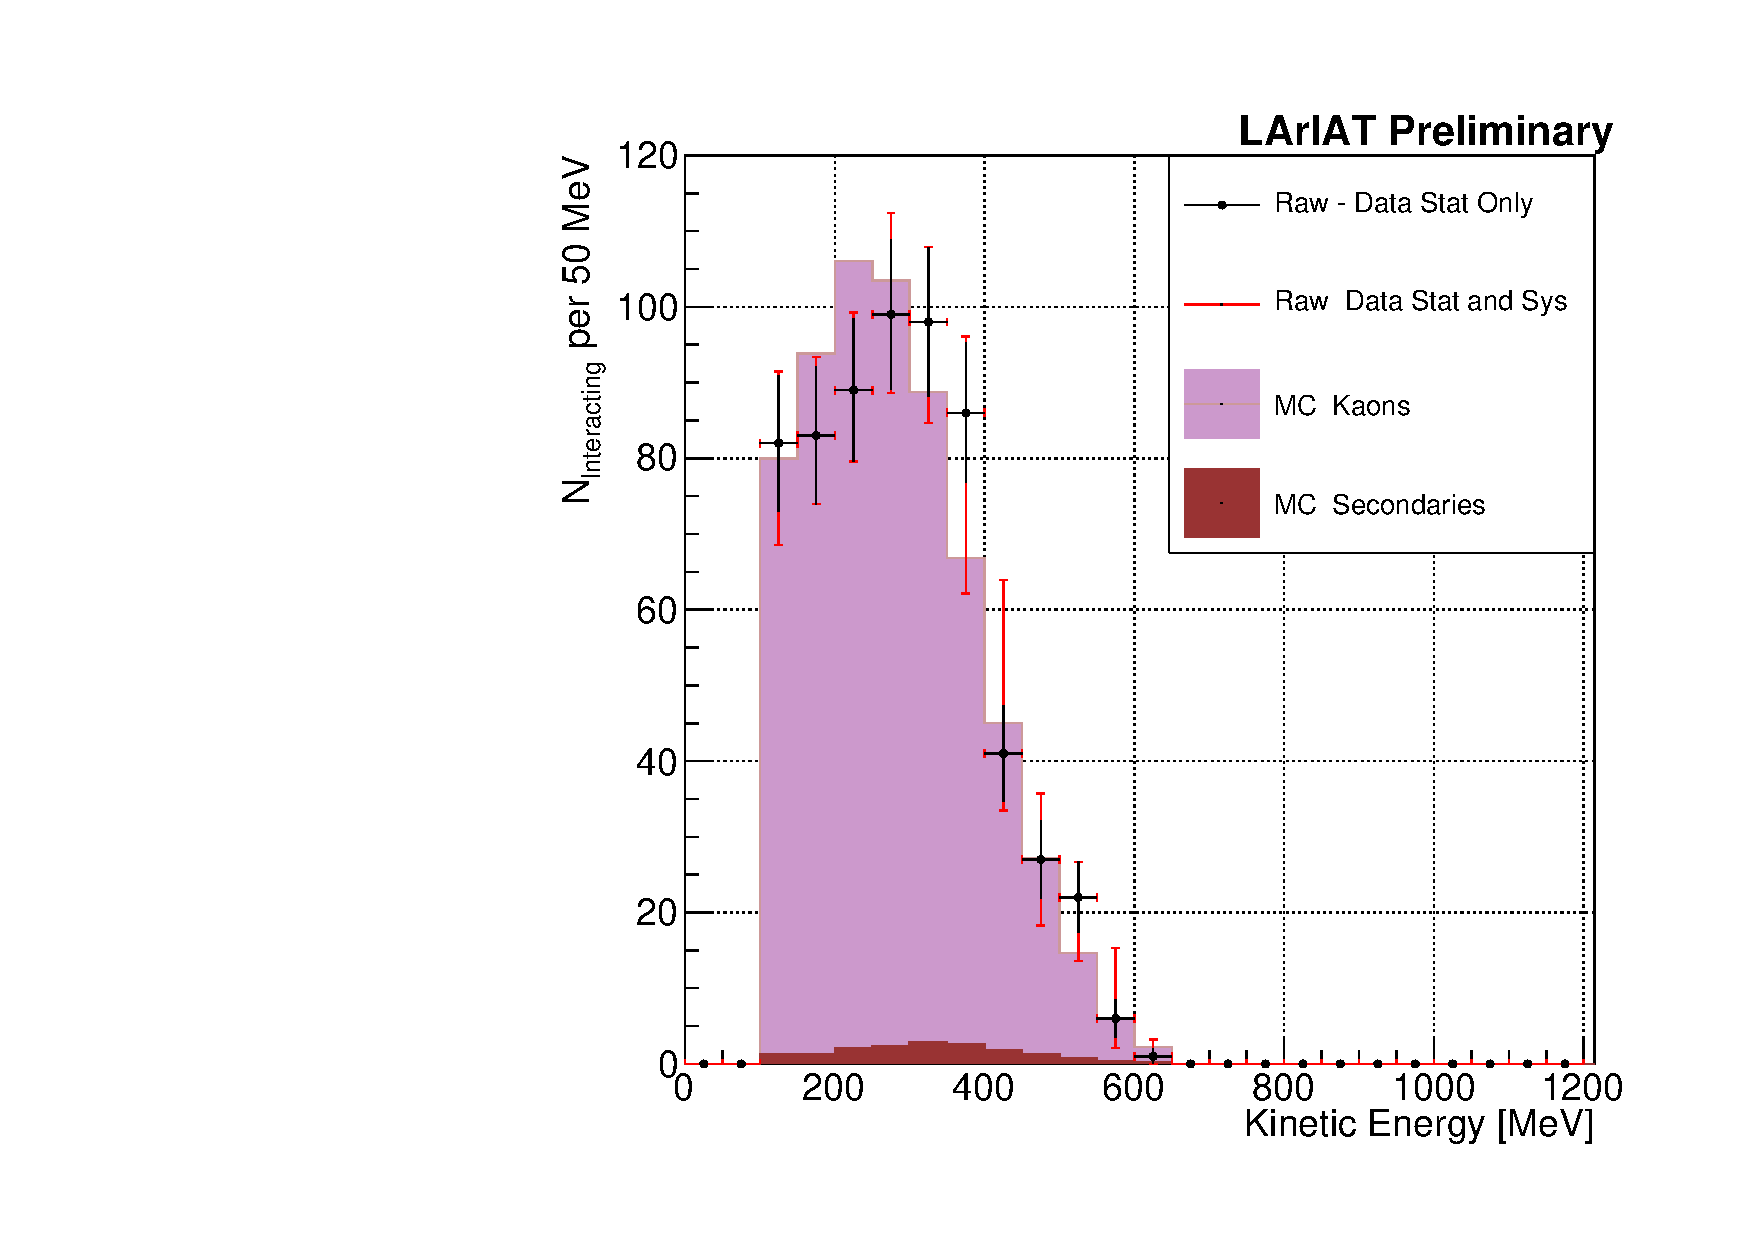
\includegraphics[width=\textwidth]{Chapter-7/Images/Plots_MCData_Int_StatSystK.pdf}
\caption{Raw number of interacting kaon candidates as a function of the reconstructed kinetic energy. The statistical uncertainties are shown in black, the systematic uncertainties in red.}
\label{fig:InteractingRawK}
\end{minipage}\hfill
\begin{minipage}[t]{0.45\textwidth}
\centering
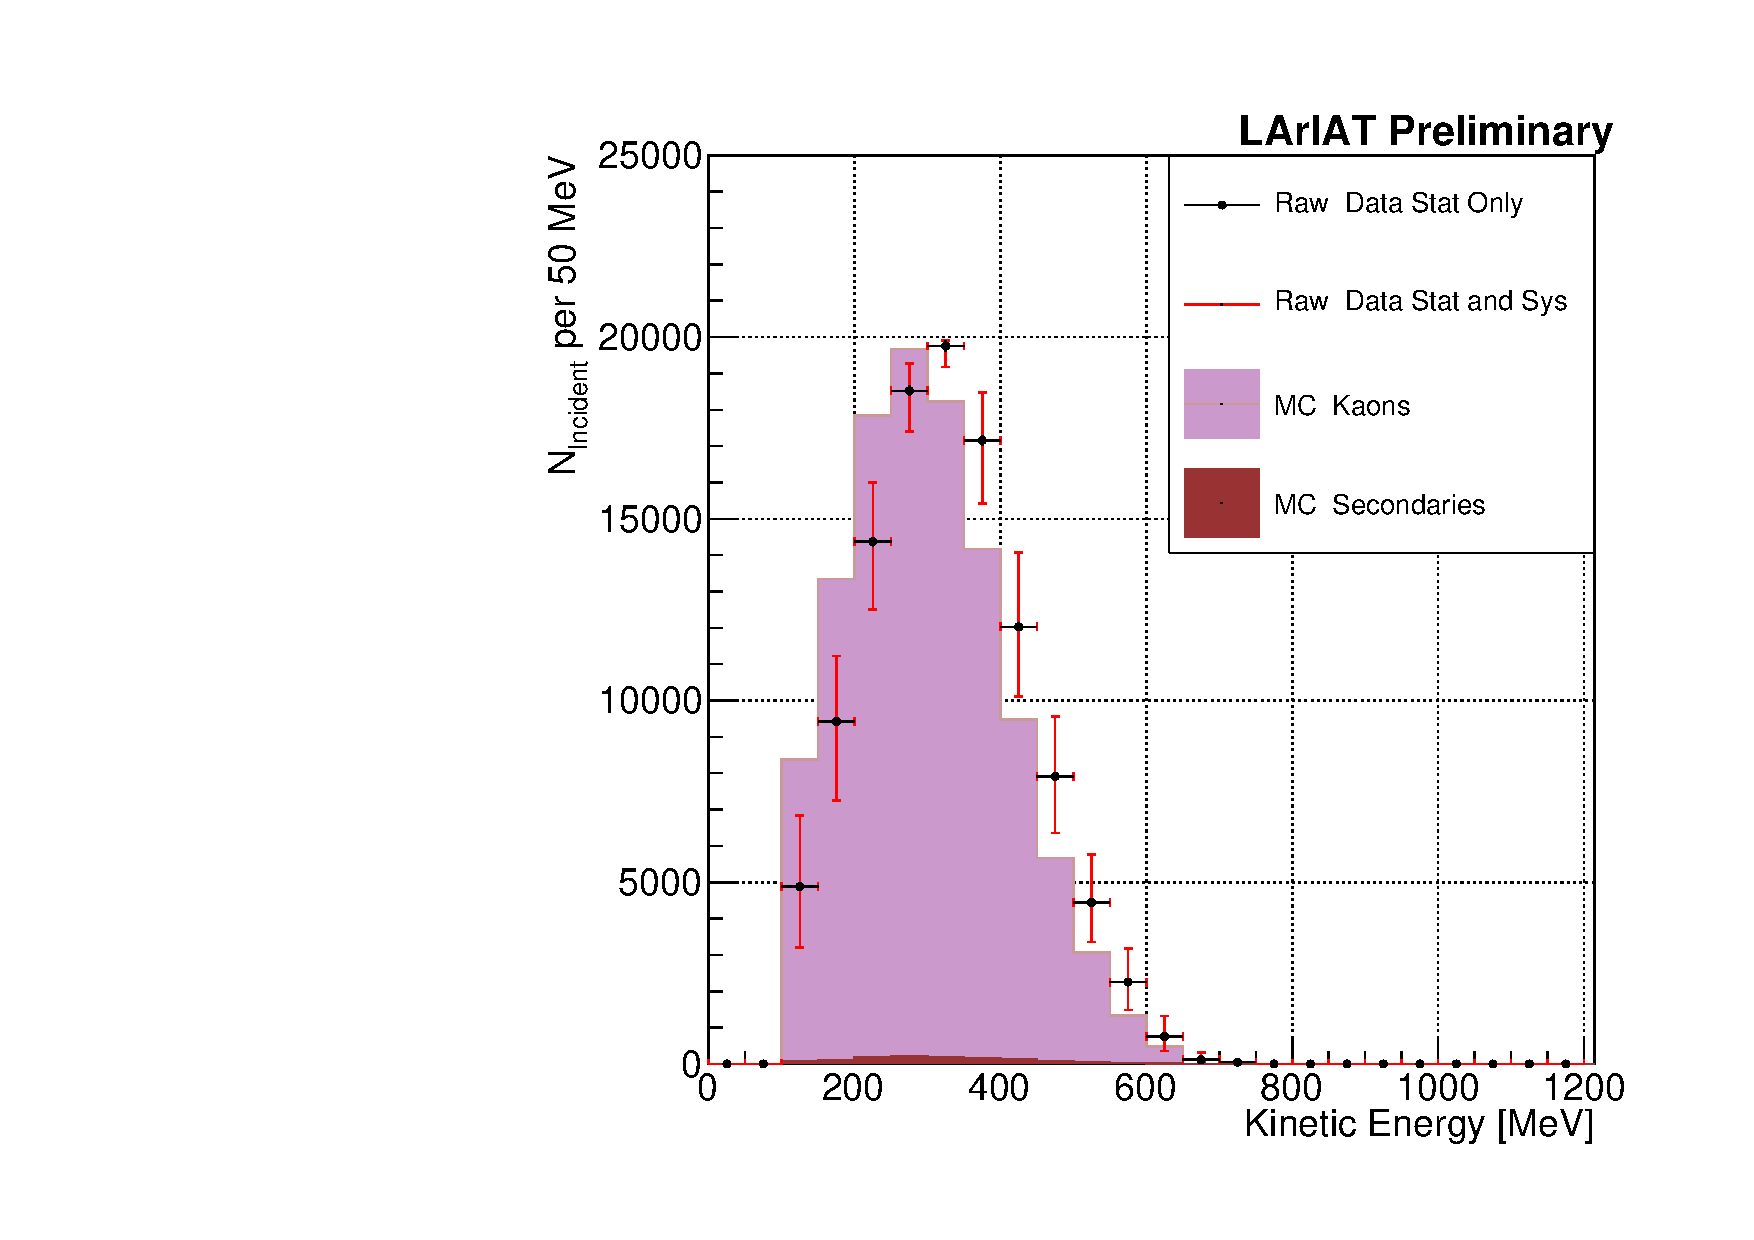
\includegraphics[width=\textwidth]{Chapter-7/Images/Plots_MCData_Inc_StatSystK.pdf}
\caption{Raw number of incident kaon candidates as a function of the reconstructed kinetic energy. The statistical uncertainty is shown in black, the systematic uncertainties in red.}
\label{fig:IncidentRawK}
\end{minipage}
\end{figure}



\begin{figure}
\centering  
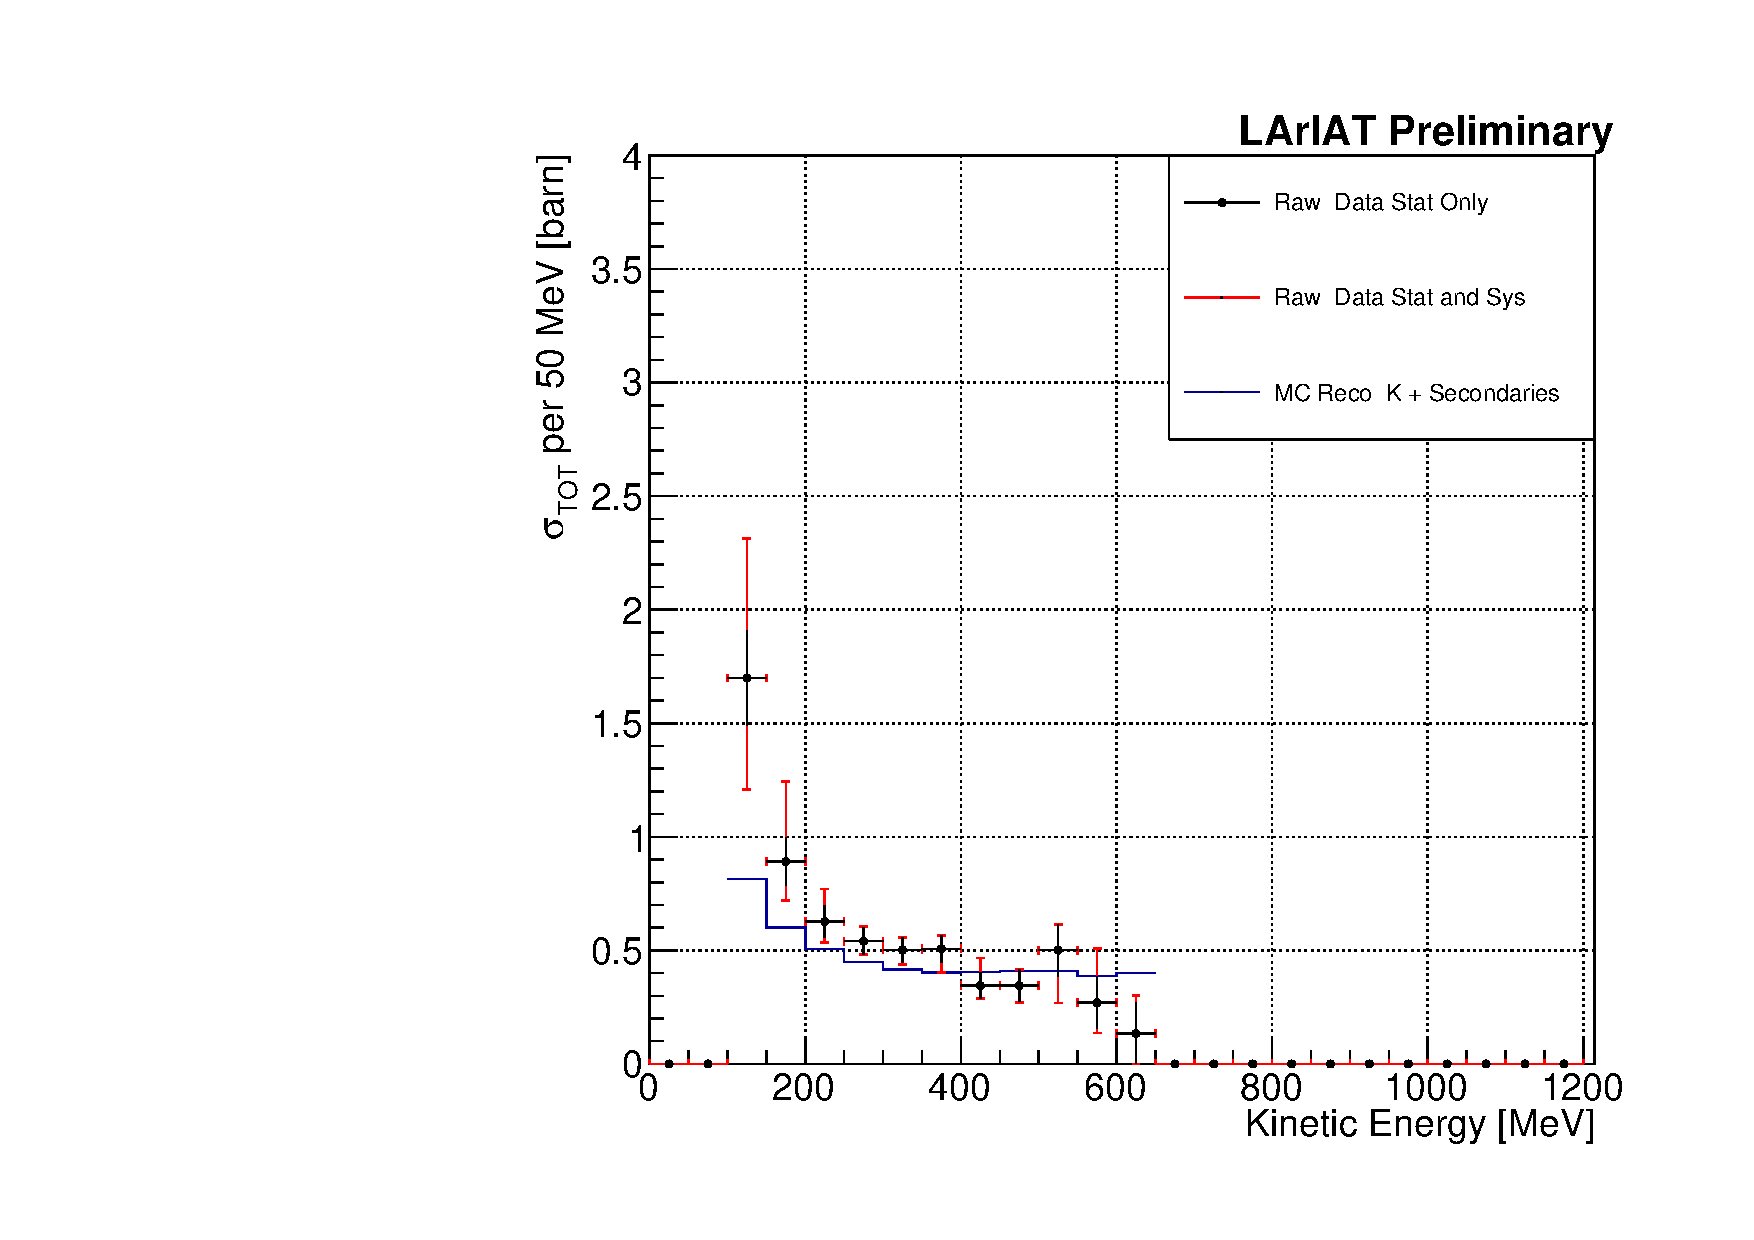
\includegraphics[width=0.48\textwidth]{Chapter-7/Images/Plots_MCData_XS_StatSystK.pdf}
\caption{Raw ($K^+$-Ar) total hadronic cross section. The statistical uncertainty is shown in black, the systematic uncertainties in red. The raw cross section obtained with a MC sample of kaons is shown in azure. For the MC cross section,  we include the contributions from secondaries. }
\label{fig:XSRaw}
\end{figure}





\begin{comment}

\section{Corrections to the Raw Cross Section}\label{ch:KaonXSCorrections}
As described in section \ref{ch:MCCorrections}, we need to apply a background correction and an efficiency correction in order to derive the true Kaon cross section from the raw cross section.  The true cross section is given in equation \ref{eq:C}, 

\begin{equation}
   \sigma^{\pi^-}_{TOT}(E_{i})  = \frac{1}{n \delta X}\frac{ \epsilon^{\text{Inc}}(E_i)  \hspace{0.2cm} C^{\pi MC}_{\text{Int}} (E_{i}) \hspace{0.2cm} N^{\text{TOT}}_{\text{Int}} (E_{i}) }{   \epsilon^{\text{Int}}(E_i) \hspace{0.2cm} C^{\pi MC}_{\text{Inc}} (E_{i}) \hspace{0.2cm}  N^{\text{TOT}}_{\text{Inc}} (E_{i})}.
 \tag{\ref{eq:C}}
\end{equation}

Section \ref{ch:BKGsubXSPuppa} describes the evaluation of Kaon content in the interacting and incident histograms, ($C^{\pi MC}_{\text{Int}} (E_{i})$  and  $C^{\pi MC}_{\text{Inc}} (E_{i})$) and the propagation to the cross section measurement of the relative systematic uncertainties.

Section \ref{ch:EFFXS} describes the procedure employed to obtain  the efficiency corrections $\epsilon^{\text{Int}}(E_i)$  and $\epsilon^{\text{Inc}}(E_i)$ and the propagation to the cross section measurement of the relative uncertainties.


\subsection{Background subtraction}\label{ch:BKGsubXSPuppa}
We use the procedure described in \ref{ch:KaonXSBkgSub2} to evaluate the relative Kaon content in the interacting histogram $C^{\pi MC}_{\text{Int}} (E_{i})$  and the relative Kaon content in the incident $C^{\pi MC}_{\text{Inc}} (E_{i})$. We start by evaluating the relative Kaon content assuming the beamline composition simulated by G4Beamline, whose Kaon, muon and electron percentages per beam condition are reported again in the first line of Table \ref{tab:beamlineSys}. The left side of Figure \ref{fig:CorrectionsBeam} shows the  MC estimated  relative Kaon content for the interacting histogram as function of kinetic energy for the 60A runs (top) and 100A runs (bottom). The right side of the same figure shows the  MC estimated  relative Kaon content for the incident histogram as function of kinetic energy for the 60A runs (top) and 100A runs (bottom). In Figure \ref{fig:CorrectionsBeam} the central curves displayed in light blue are obtained using the beamline composition as predicted by G4Beamline: these are the correction curves for the relative Kaon content applied to data.

So, the question now becomes: how well do we know the beamline composition? In absence of additional data constraints,  we take a 100\% systematic uncertainty on the electron content, reported in lines 3 and 4 of Table \ref{tab:beamlineSys}. The effect of doubling or halving the electron percentage in the beam on the Kaon relative content is displayed in red in Figure \ref{fig:CorrectionsBeam}. We reserve a slightly different treatment for the muon content. Since G4Beamline tracks only particles which cross all the wire chambers, Kaon events that decay in flight from WC1 to WC4 are not recorded by G4Beamline. Kaon decays in the beamline could be trigger the beamline detectors in data, if the produced muon proceeds in the beamline. Thus, we take the G4Beamline prediction for muons as a lower bound in the composition: the effect of doubling the muon content (line 2 in Table \ref{tab:beamlineSys}) is shown in blue on Figure \ref{fig:CorrectionsBeam}. A future study of data from additional beamline detectors such as the Aerogel Chernkov detectors \cite{detectorPaper} or the muon range stack (see Section \ref{sec:MuRS}) has the potential of a narrowing the systematics uncertainty coming from the beamline compositon.


We propagate the uncertainty on the beamline composition  as a systematic uncertainty to the cross section by varying the beam composition for all the cases listed in Table \ref{tab:beamlineSys} and evaluating variation of obtained  data cross sections in each bin. This systematic uncertainty is summed in quadrature with the statistical uncertainty and the systematic uncertainty related to the kinetic energy measurement.


\begin{table}[p]
\centering
\begin{tabular}{| l | l | l | l | l | l | l | l | }
\hline
 &  \multicolumn{3}{|c|}{Magnet Current -60A} & \multicolumn{3}{|c|}{Magnet Current -100 A}\\

                                                  & MC $\pi^-$   & MC  $ \mu^-$ & MC  $e^-$ & MC  $\pi^-$ & MC  $\mu^-$ & MC  $e^-$  \\
\hline
Expected Composition          & 68.8	\%&4.6 \%&	26.6 \%&	87.4 \%&	3.7	\%&8.9 \% \\
Composition 2x Muons          & 64.2	\%&9.2 \%&	26.6 \%&	83.7 \%&	7.4	\%&8.9 \% \\
Composition 2x Electrons      &42.2	\%&4.6 \%&	53.2 \%&	78.5	\%&  3.7	\%&17.8 \%\\
Composition 0.5x Electrons   &82.1	\%&4.6 \%&	13.3 \%&	91.9 \%&	3.7	\%&4.4 \% \\
\hline
\end{tabular}
\caption{Beam composition variation for the study of systematics due to beam contamination.}
\label{tab:beamlineSys}
\end{table}

\begin{figure}[p]
\centering
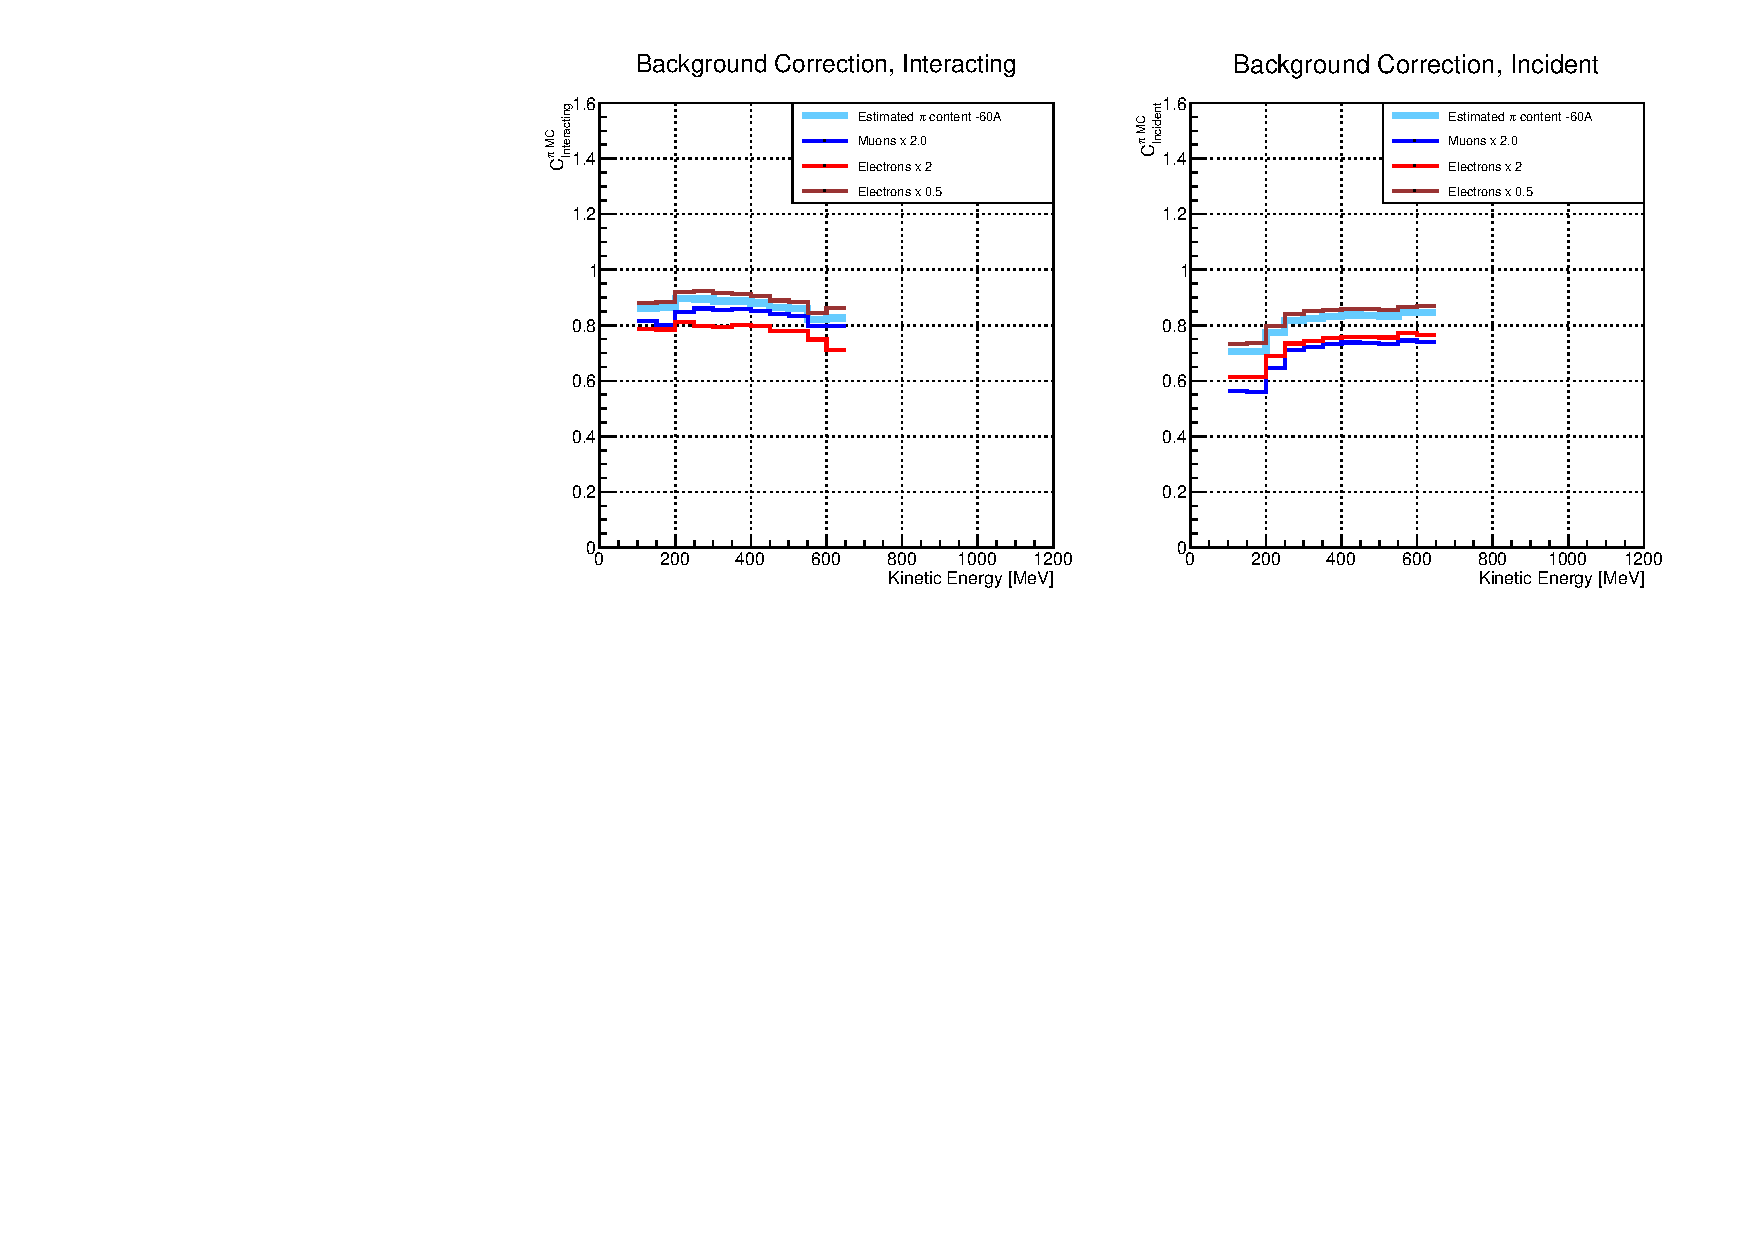
\includegraphics[width=\textwidth]{Chapter-6/Images/Bkg60A_inc_int.pdf}
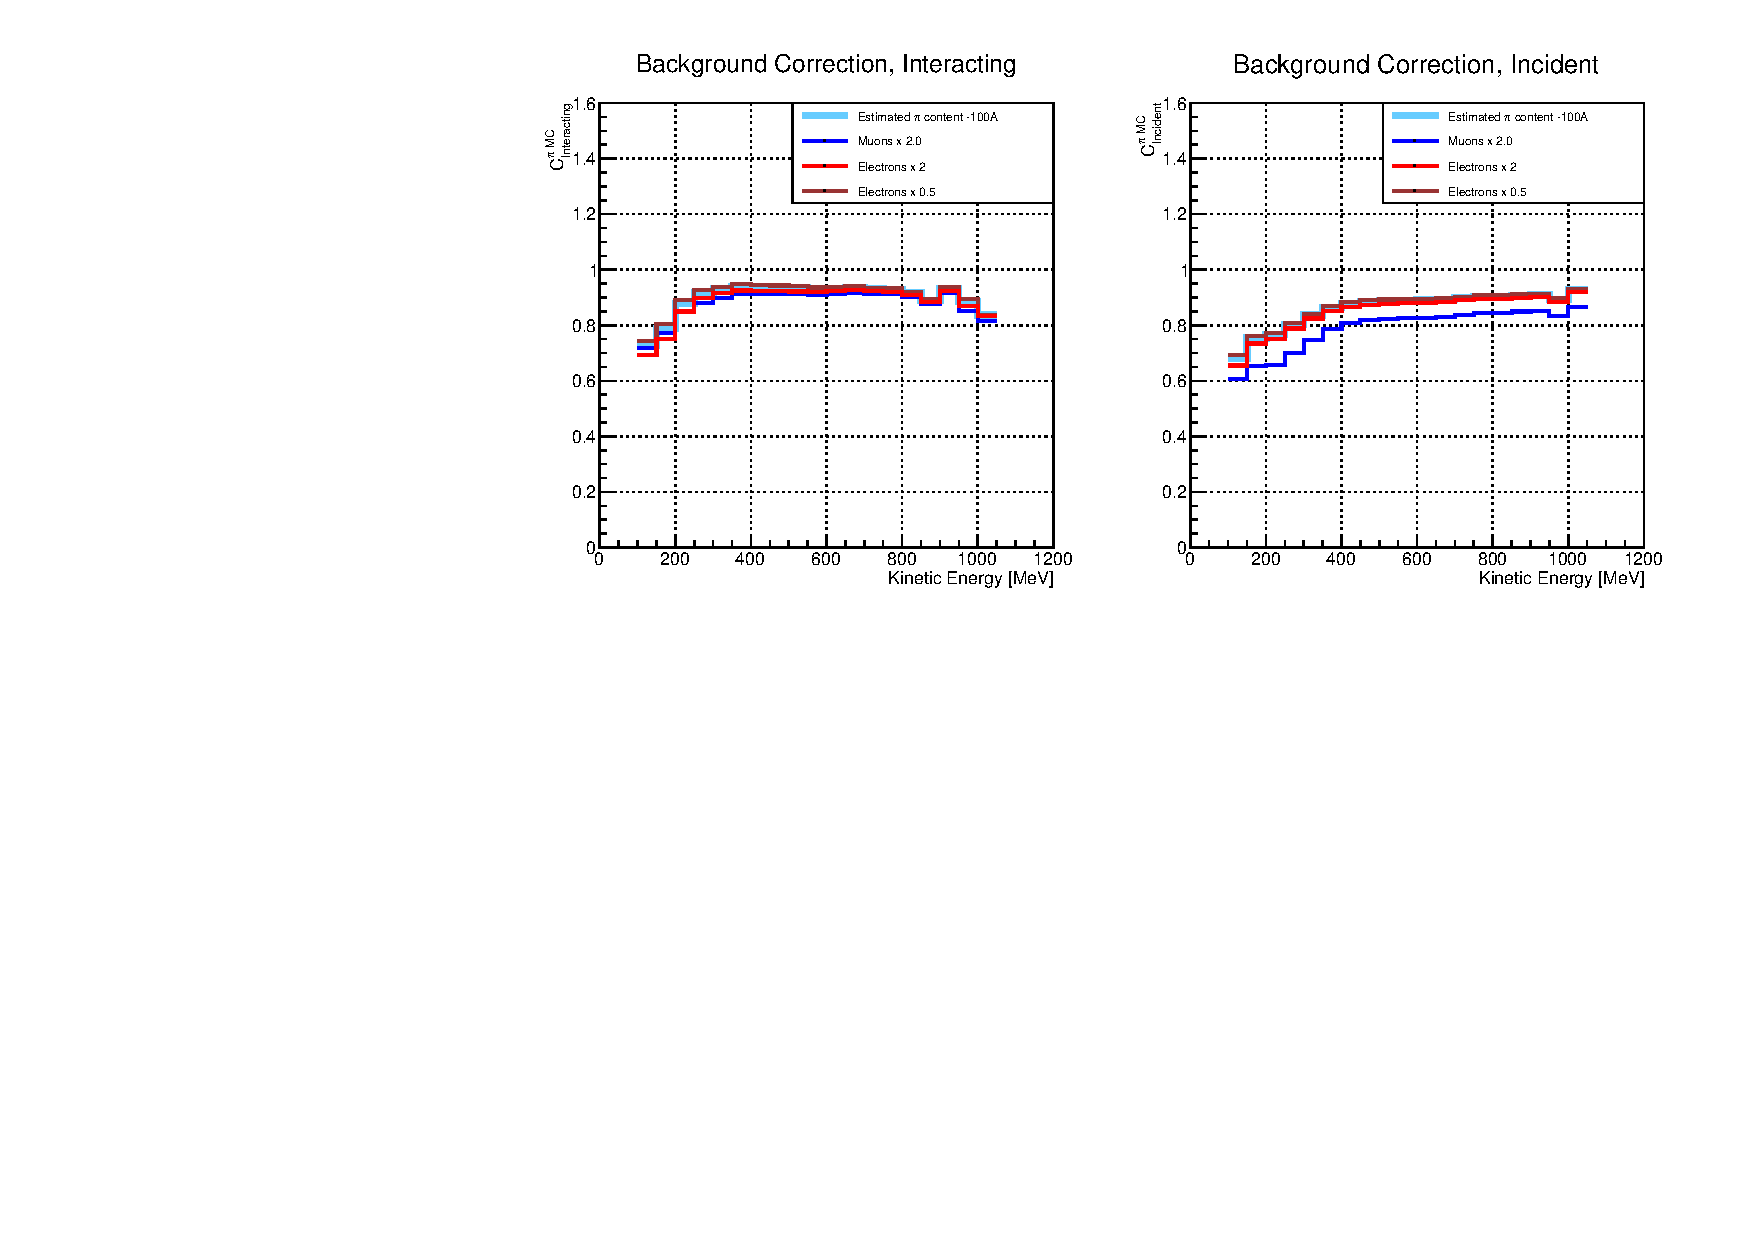
\includegraphics[width=\textwidth]{Chapter-6/Images/Bkg100A_inc_int.pdf}
\caption{\emph{Left:} MC estimated relative Kaon content for interacting histogram a function of kinetic energy for the 60A runs (top) and 100A runs (bottom), statistics uncertainty in azure and systematic uncertainty in blue. \emph{Right:}  MC estimated relative Kaon content  for incident histogram a function of kinetic energy for the 60A runs (top)  and 100A (bottom), statistics uncertainty in azure and systematic uncertainty in blue.}
\label{fig:CorrectionsBeam}
\end{figure}



\subsection{Efficiency Correction}\label{ch:EFFXS}
The interaction point for a track used in the total hadronic cross section analysis is defined to be the last point of the WC2TPC matched track which lies inside the fiducial volume. This definition is independent from the topology of the interaction. If the TPC track stops within the fiducial volume, its last point will be the interaction point, no matter what the products of the interaction look like; if the track crosses the boundaries of the fiducial volume, the track will be considered ``through going" and no interaction point will be found.  Given this definition, it is evident that we rely on the tracking algorithm to discern where the interaction occurred in the TPC  and correctly stop the tracking. The tracking algorithm has an intrinsic angle resolution as shown in section \ref{sec:angleRes}, which limits its efficiency, especially in the case of elastic scattering occurring a low angles. 
Thus, we need to apply an efficiency correction to data in order to retrieve the true cross section.  The efficiency correction is evaluated separately for the interacting and incident histograms, namely $\epsilon^{\text{int}}_i$ and  $\epsilon^{\text{inc}}_i$, and propagated to the cross section as shown in  equation \ref{eq:C}. 

\subsubsection{Efficiency Correction: Procedure}\label{sec:EffCorrection}
We describe here the procedure to calculate the efficiency correction taking the interacting histogram as example and noting that the procedure is identical for the  incident histogram. 

We derive the correction on a set of pure Kaon MC, calculating its value bin by bin as the ratio between the true bin content and the correspondent reconstructed bin content. The correction is then applied to the relevant bin in data. In formulae, the efficiency correction is calculated to be

\begin{equation}
 \epsilon^{\text{Int}}(E_i)  =  \frac{N^{\text{ $\pi$ Reco MC}}_{\text{Interacting}} (E_{i})}{ N^{\text{ $\pi$ True MC}}_{\text{Interacting}} (E_{i})  },
\end{equation}
 
where $N^{\text{ $\pi$ True MC}}_{\text{Int}} (E_{i}) $ is the content of the $i$-th bin in for the true interacting histogram, and $N^{\text{ $\pi$ Reco MC}}_{\text{Int}} (E_{i}) $ is the content of the $i$-th bin in for the reconstructed interacting histogram. The correction is applied to data as follows

\begin{equation}
N^{\text{ $\pi$ True Data}}_{\text{Int}} (E_{i})  =  \frac{N^{\text{$\pi$ Reco Data}}_{\text{Int}} (E_{i})}{\epsilon^{\text{Int}} (E_{i}) } = N^{\text{$\pi$ Reco Data}}_{\text{Int}} (E_{i}) \frac{N^{\text{ $\pi$ True MC}}_{\text{Int}} (E_{i})}{ N^{\text{ $\pi$ Reco MC}}_{\text{Int}} (E_{i})}.
\end{equation}

where $N^{\text{$\pi$ Reco Data}}_{\text{Int}} (E_{i})$ is the background subtracted bin content of the $i$-th bin in for the reconstructed interacting histogram for data, i.e. 
\begin{equation}
N^{\text{$\pi$ Reco Data}}_{\text{Int}} (E_{i}) =  N^{\text{TOT Data}}_{\text{Int}} (E_{i}) - B^{\text{Data}}_{\text{Int}} (E_i)  =  C^{\text{$\pi$ MC}}_{\text{Int}} (E_{i}) N^{\text{TOT Data}}_{\text{Int}} (E_{i}).
\end{equation}


In section \ref{sec:angleRes}, we estimated the angular resolution for data and MC to be $\bar\alpha_{Data} = (5.0 \pm 4.5) \text{ deg}$  and 
$\bar\alpha_{MC} = (4.5 \pm 3.9) \text{ deg}$, respectively.  Most interaction angles smaller than the angular resolution will thus be indistinguishable  for the reconstruction. Thus, we claim we are able to  measure the cross section for interaction angles greater than 5.0 deg. Geant4 simulates interactions at all angles, as shown in figure \ref{fig:trueScatteringAngle}. In order to calculate the efficiency correction,  we select events which have an interaction angle greater than a given $\alpha_{res}$ to construct the true interacting and incident histograms (the denominator of the efficiency correction). The systematics on the efficiency correction is estimated by varying the value of $\alpha_{res}$ between 0 deg and 4.5 deg and propagating the uncertainty on the cross section. 


Figure \ref{fig:EffCorr60A} shows $\epsilon^{\text{Int}}(E_{i})$ in the left side and $ \epsilon^{\text{Inc}}(E_i)$ on the right as a function of the kinetic energy for the 60A runs and their systematic uncertainty. Similarly, figure \ref{fig:EffCorr100A} shows $\epsilon^{\text{Int}}(E_{i})$ in the left side and $ \epsilon^{\text{Inc}}(E_i)$ on the right as a function of the kinetic energy for the 100A runs and their systematic uncertainty. 

\begin{figure}[p]
\centering
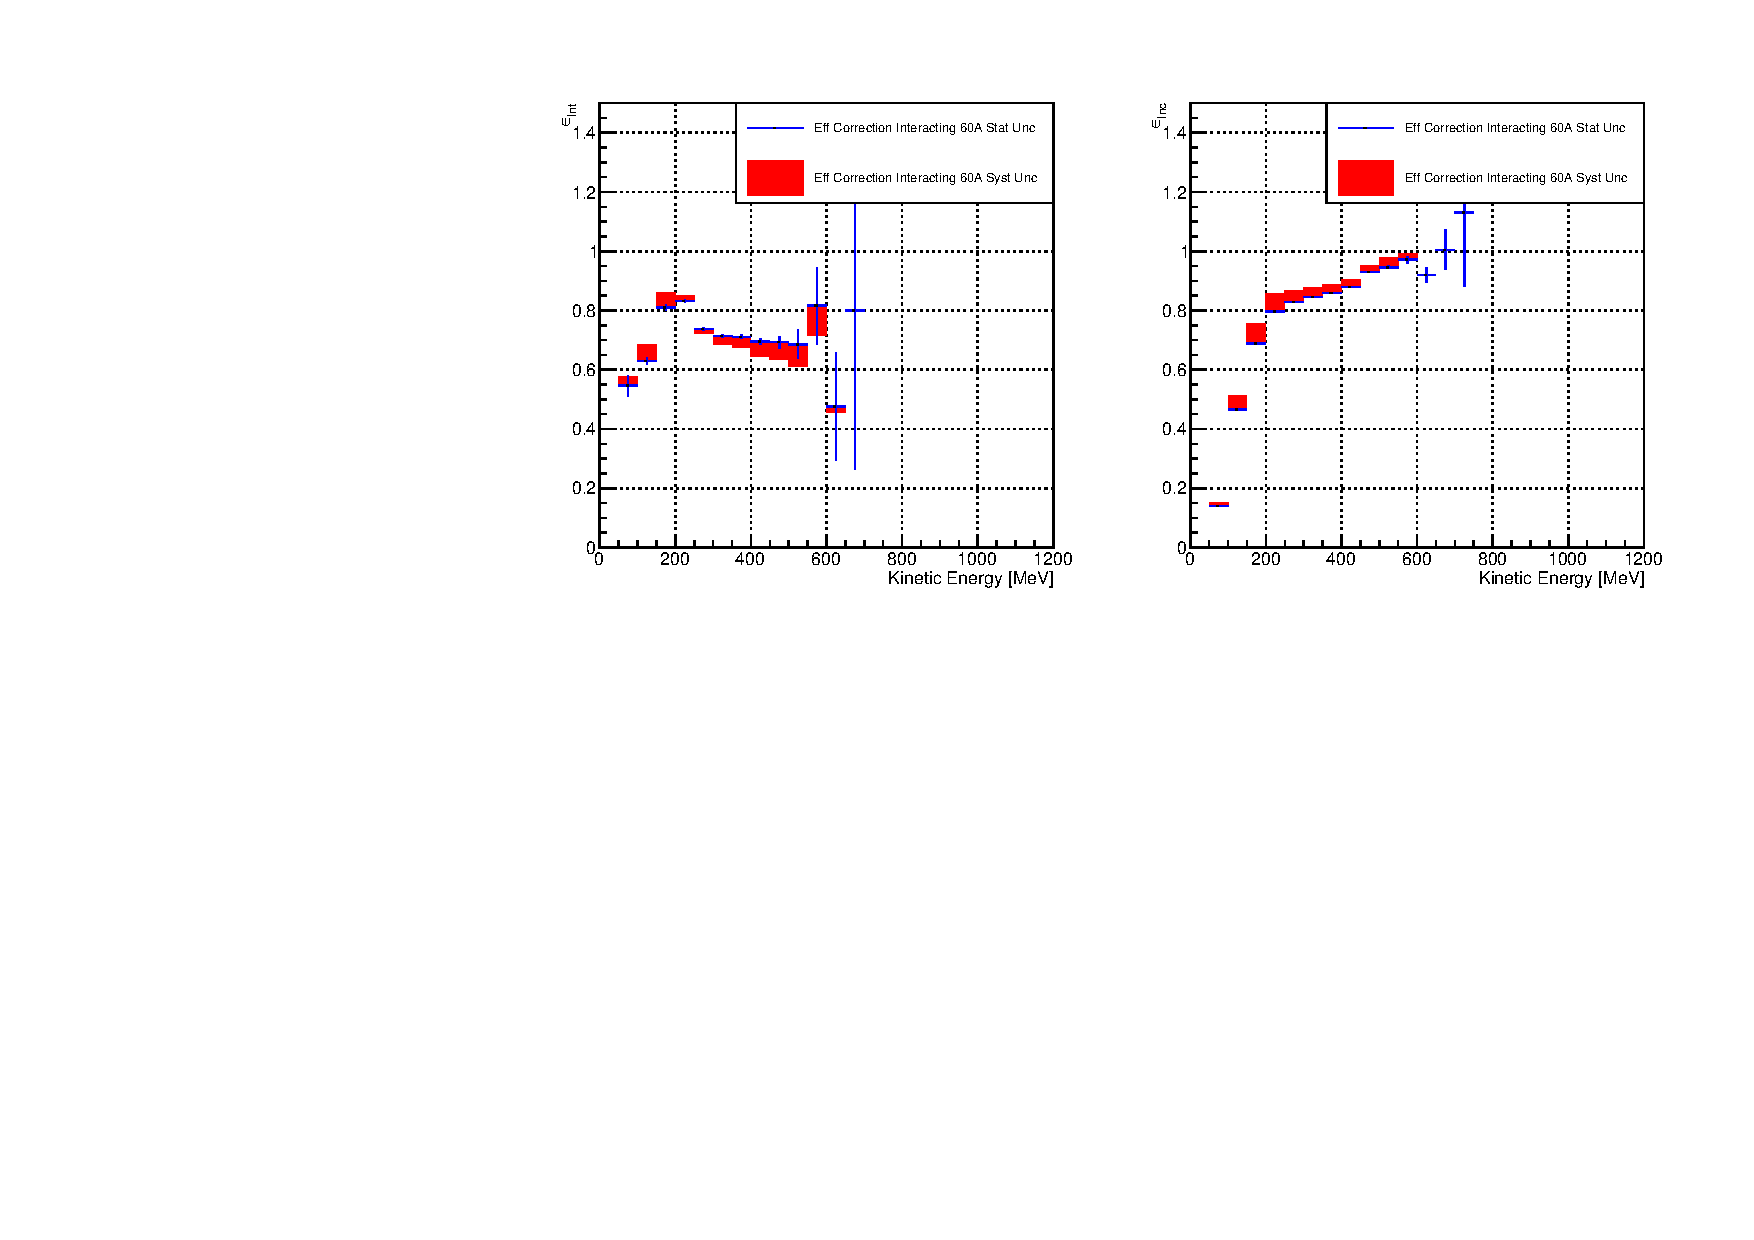
\includegraphics[width=\textwidth]{Chapter-6/Images/60AEffCorr.pdf}
\caption{\emph{Left:} Efficiency correction on the 60A interacting histogram, statistical uncertainty in blue, systematic uncertainty in red. \emph{Right:}  Efficiency correction on the 60A incident histogram, statistical uncertainty in blue, systematic uncertainty in red.}
\label{fig:EffCorr60A}
\end{figure}

\begin{figure}[p]
\centering
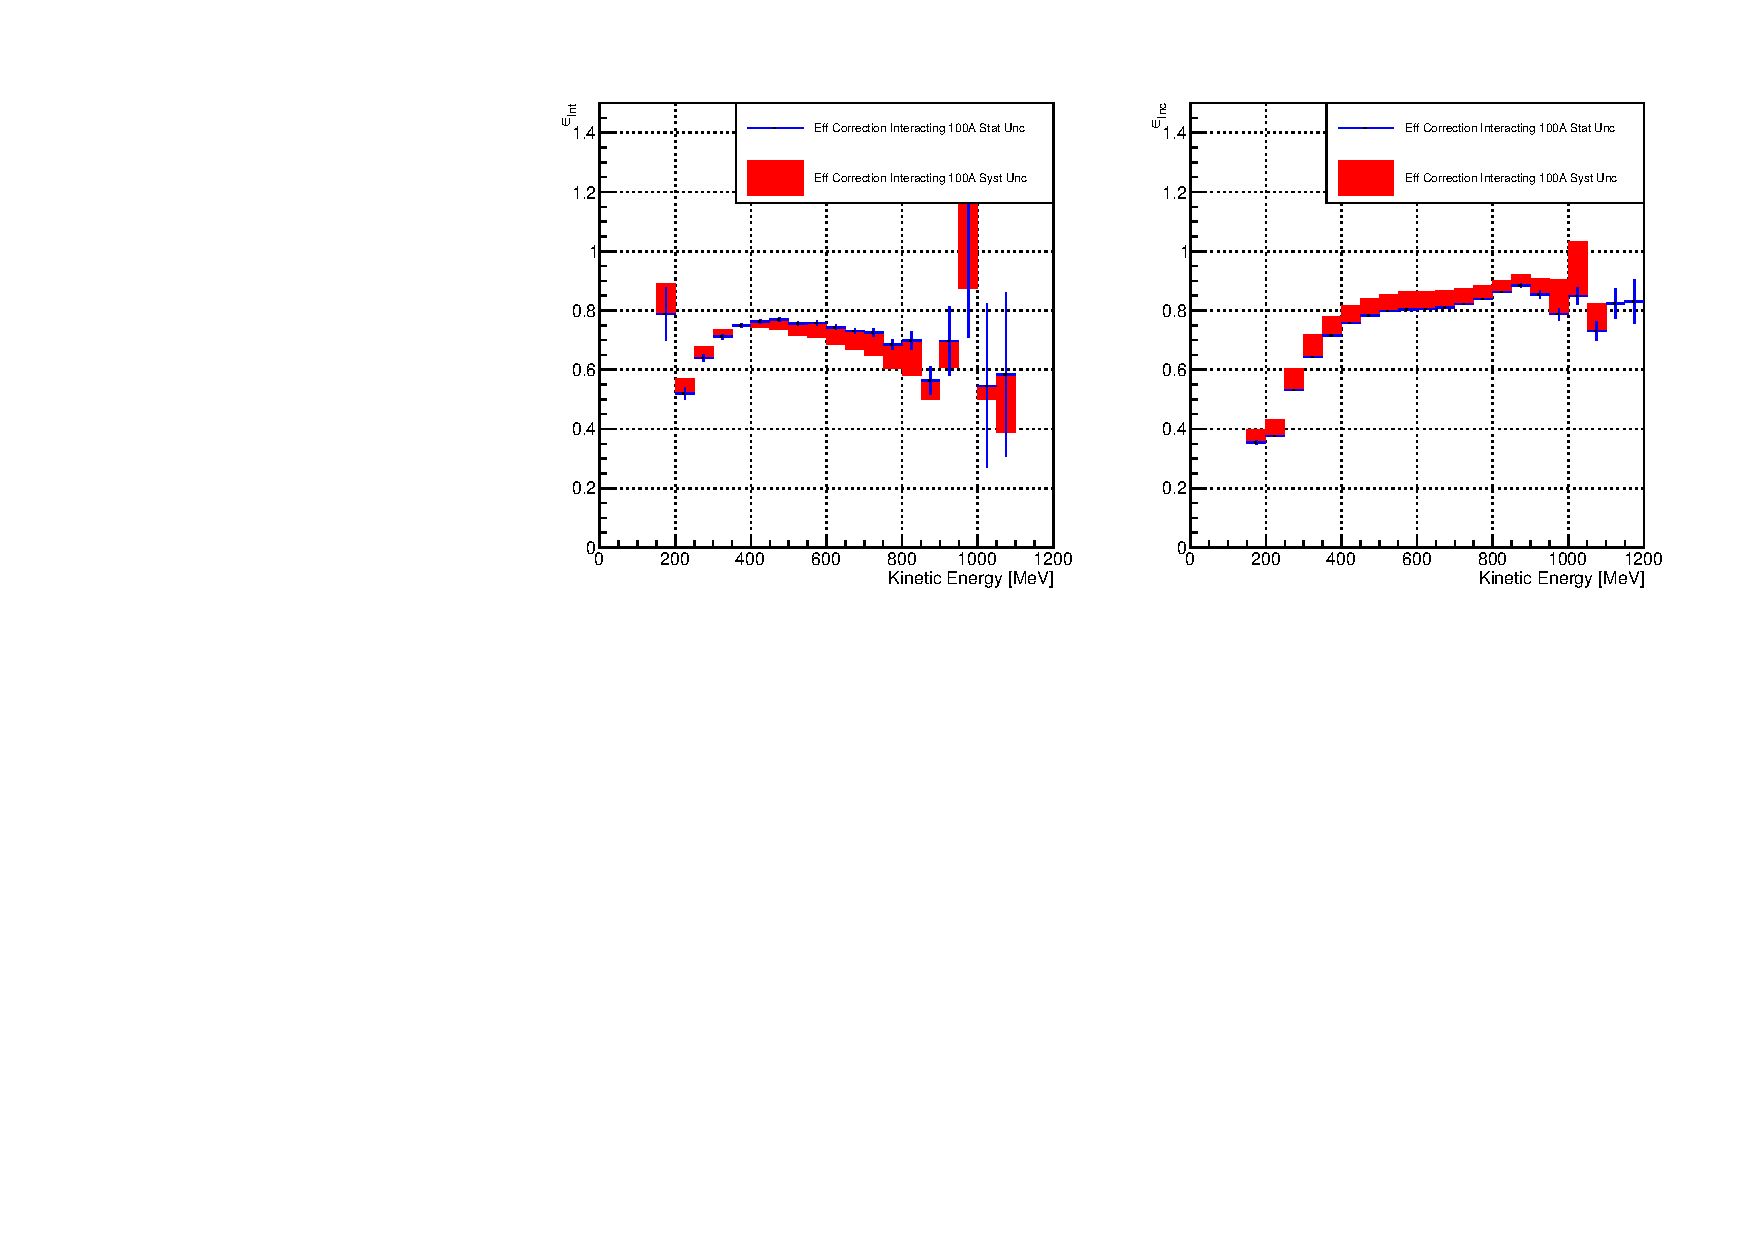
\includegraphics[width=\textwidth]{Chapter-6/Images/100AEffCorr.pdf}
\caption{\emph{Left:} Efficiency correction on the 100A interacting histogram, statistical uncertainty in blue, systematic uncertainty in red. \emph{Right:}  Efficiency correction on the 100A incident histogram, statistical uncertainty in blue, systematic uncertainty in red.}
\label{fig:EffCorr100A}
\end{figure}



\begin{figure}[p]
\centering
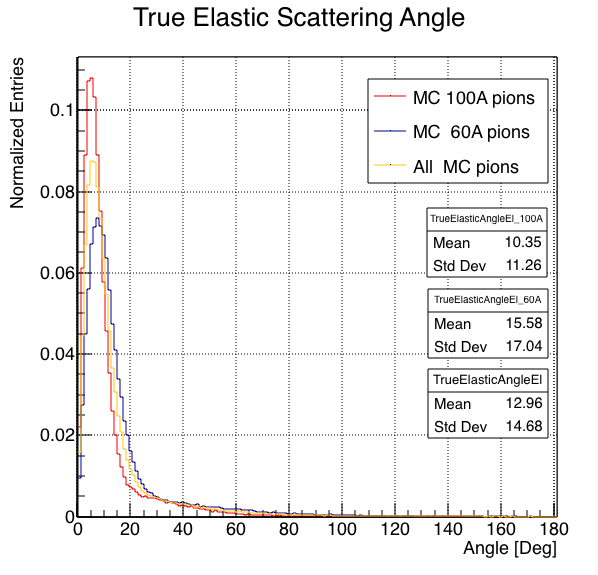
\includegraphics[width=0.48\textwidth]{Chapter-5/Images//cAngleTrue.png}
\caption{Distribution of the true scattering angle for a Kaon elastic scattering off the argon nucleus as simulated by Geant4.}
\label{fig:trueScatteringAngle}
\end{figure}




\clearpage
\section{Results}\label{ch:FinalKaon}
Figure \ref{fig:FinalXSKaon} show the measurement of the ($\pi^-$-Ar) total hadronic cross section for  scattering angles greater than 5$^\circ$, as the result of the background subtraction and efficiency correction to the raw cross section. The top left plot is the measurement obtained on the 60A data, statistical uncertainty in black and systematic uncertainty in red. The top right plot is the measurement obtained on the 100A data, statistical uncertainty in black and systematic uncertainty in blue. The bottom plot shows the two measurements overlaid. In all three plot, the Geant4 prediction for the total hadronic cross section for angle scattering greater than 5$^\circ$ is displayed in green.

The systematic uncertainty on the cross section is the sum in quadrature of the statistical uncertainty, the systematic uncertainty related to the kinetic energy measurement, the systematic uncertainty related to the beam composition and the systematic uncertainty related to the efficiency correction.

\begin{figure}[htb]
\centering
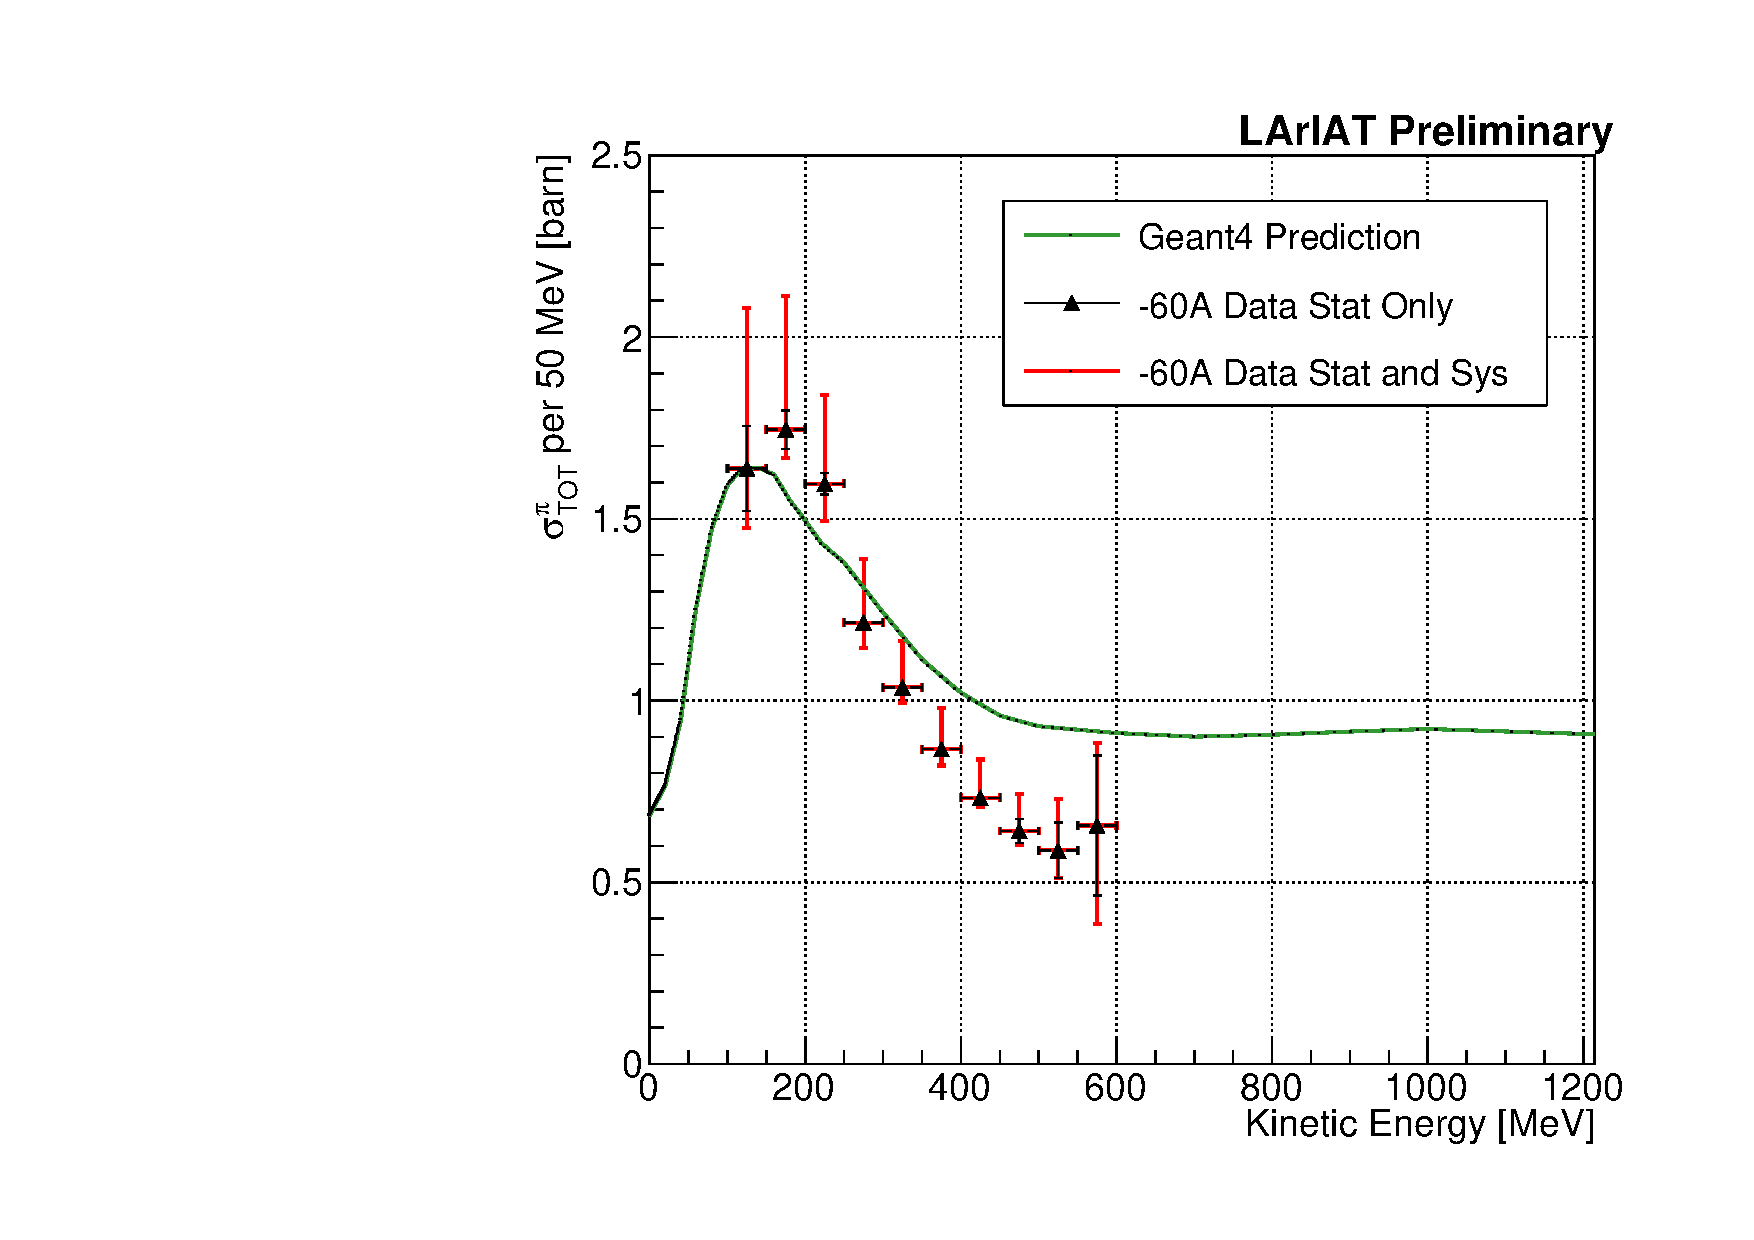
\includegraphics[width=0.48\textwidth]{Chapter-6/Images/TheMoneyPlot60A.pdf}
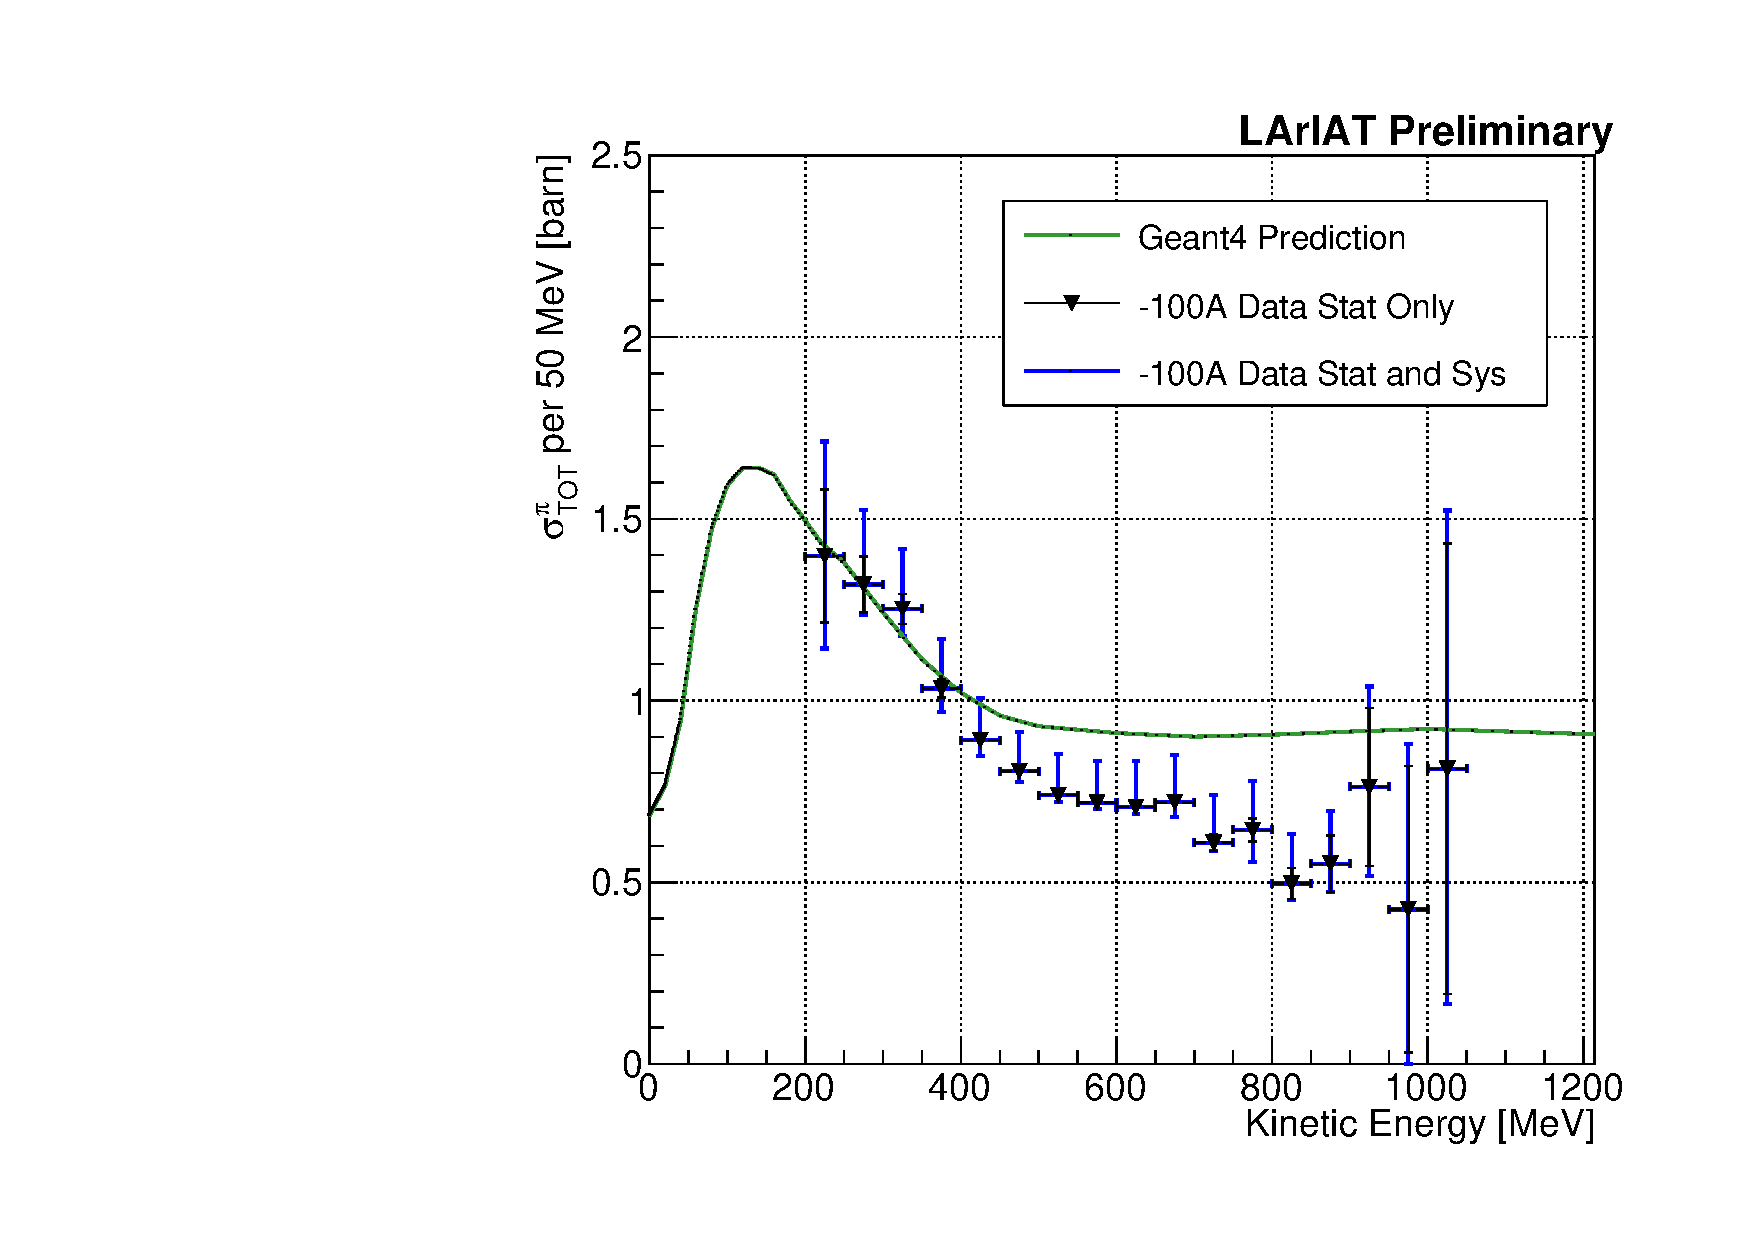
\includegraphics[width=0.48\textwidth]{Chapter-6/Images/TheMoneyPlot100A.pdf}
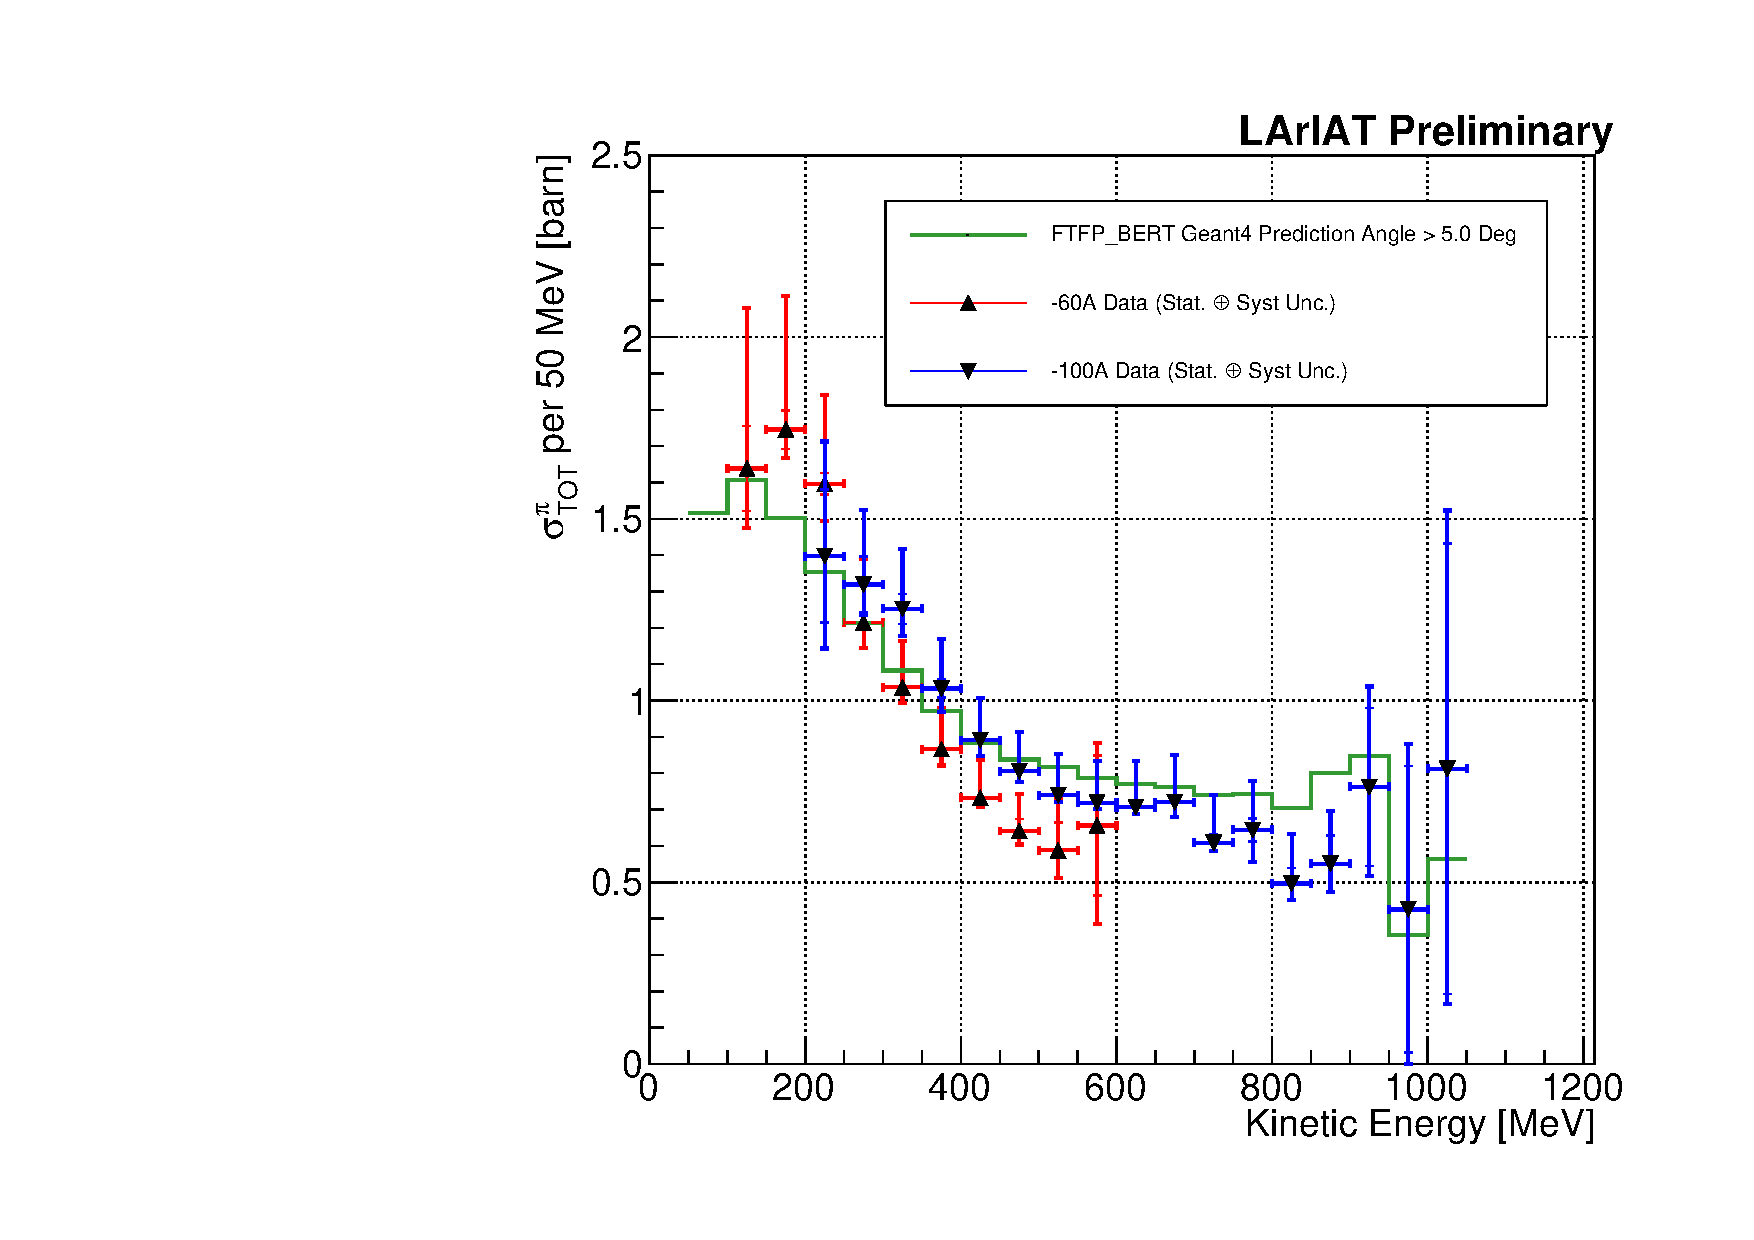
\includegraphics[width=0.48\textwidth]{Chapter-6/Images/TheMoneyPlot.pdf}
\caption{ \emph{Top Left:} ($\pi^-$-Ar) total hadronic cross section for  scattering angles greater than 5$^\circ$ measured in the 60A sample, statistical uncertainty in black and systematic uncertainty in red. The Geant4 prediction for the total hadronic cross section for angle scattering greater than 5$^\circ$ is displayed in green. \\ 
\emph{Top Right:} ($\pi^-$-Ar) total hadronic cross section for  scattering angles greater than 5$^\circ$ measured in the 100A sample, statistical uncertainty in black and systematic uncertainty in blue. The Geant4 prediction for the total hadronic cross section for angle scattering greater than 5$^\circ$ is displayed in green.\\
\emph{Bottom:} ($\pi^-$-Ar) total hadronic cross section measurements in the 60A and 100A samples overlaid with the  Geant4 prediction (green).}
\label{fig:FinalXSKaon}
\end{figure}

\subsection{Background subtraction}\label{ch:BKGsubXS}


\subsection{Background Contribution to the Cross Section}\label{sec:Correction}



\subsubsection{Treatment of Systematics}


\end{comment}

